%!TEX TS-program = xelatex
\documentclass[slidescentered]{beamer}
\usepackage{color}
\usetheme{Berkeley}
\usecolortheme{whale}

\newsavebox{\authbox}
\sbox{\authbox}{%
\centering
\begin{minipage}{0.45\linewidth}
\centering\normalsize
Candidato \par
Michele Gorini
\end{minipage}
\hfill
\begin{minipage}{0.45\linewidth}
\centering\normalsize
Relatore \par
prof. Roberto Paoletti
\end{minipage}
}

\title{Orbite periodiche di flussi Hamiltoniani su ipersuperfici convesse}
\author[Michele Gorini]{%
\usebox{\authbox}
}
\institute[Unimib]{Università degli studi di Milano-Bicocca}
\date{26 Novembre 2015}
\logo{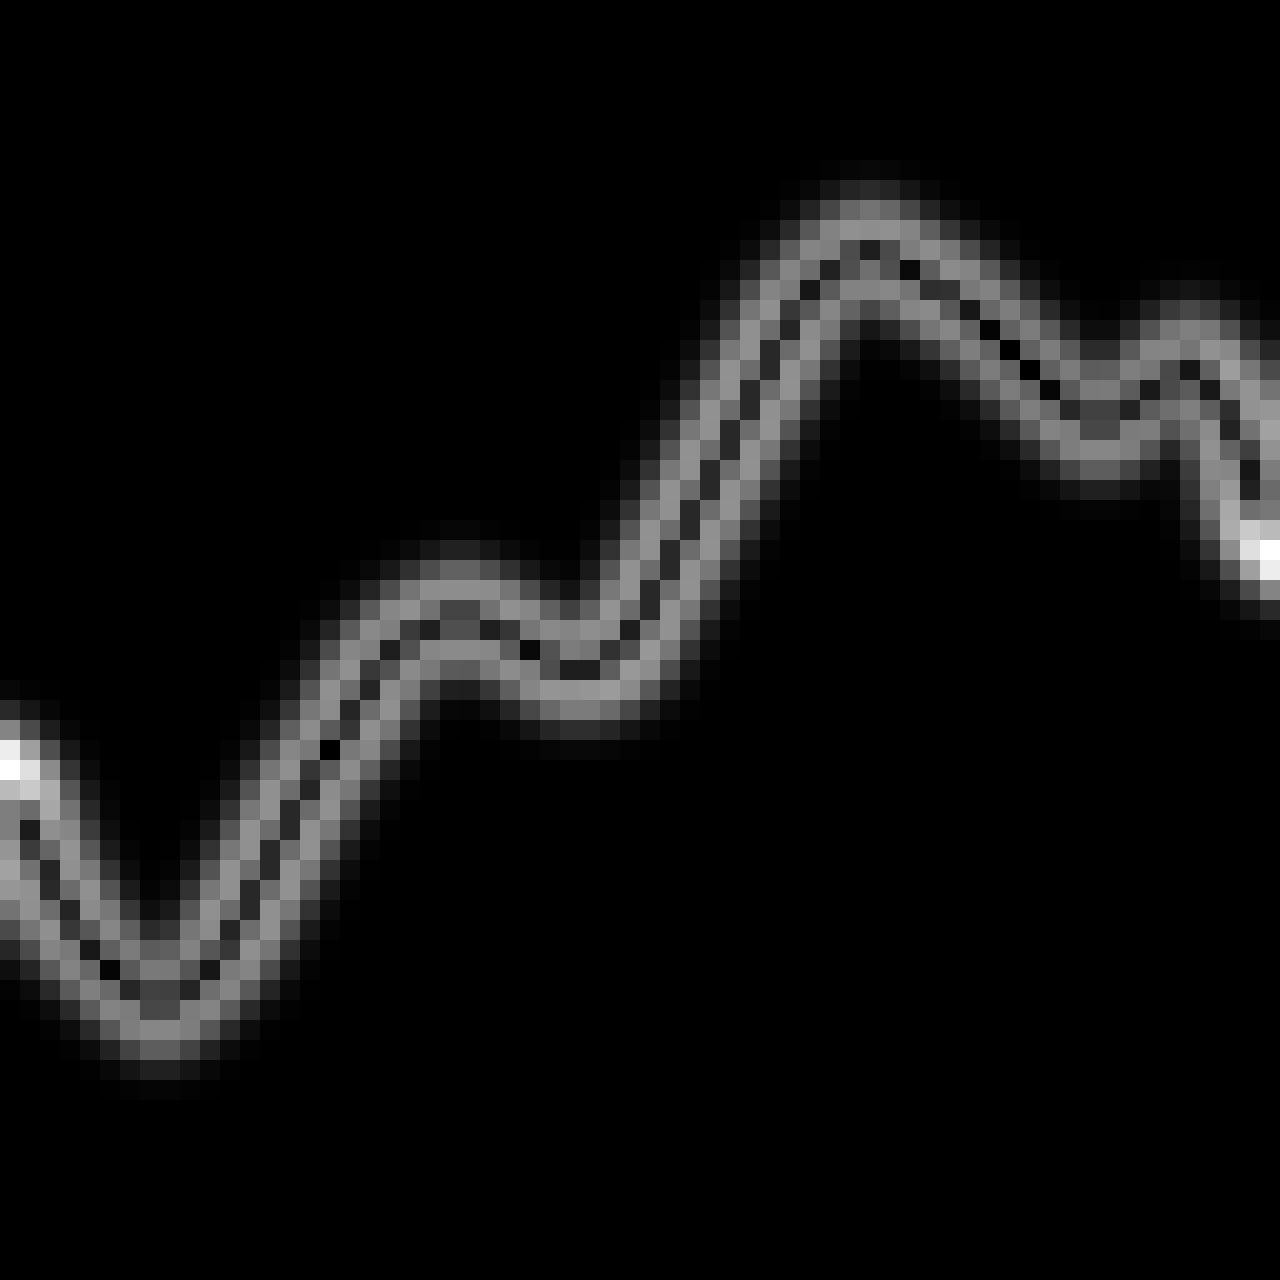
\includegraphics[width=1cm]{gradients.png}}

\begin{document}

\begin{frame}
\titlepage
\end{frame}

    \begin{frame}
        \frametitle{Outline}
        \tableofcontents{}
    \end{frame}
    
    
    \section{Introduction}
    \begin{frame}
        \frametitle{Introduction}
        \begin{center}
            \begin{itemize}
                \item BCI challenging technology.
                \item Outstanding advances but yet its push into mainstream technology has not fully materialized.
                \item More clinical and physician Involvement: devise mechanisms to help them stay in the loop.
            \end{itemize}
        \end{center}
    \end{frame}

\end{document}